
\section{Experiments}

\subsection{Synthetic experiments}

\begin{figure*}[t]
\hfill
\begin{subfigure}[b]{.325\linewidth}
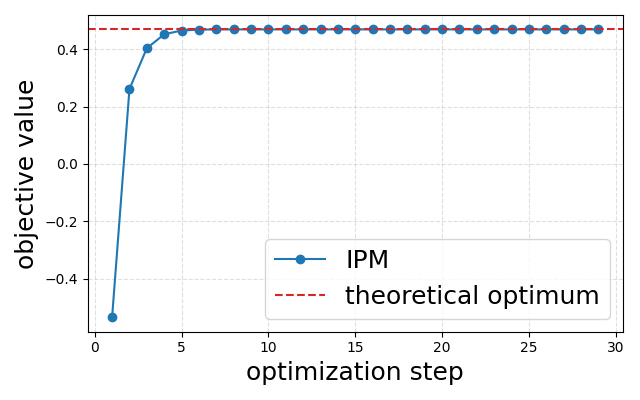
\includegraphics[width=\linewidth]{figs/obective_curve_p=0.2.png}
\subcaption{$p = 0.2$}
\end{subfigure}
\hfill
\begin{subfigure}[b]{.325\linewidth}
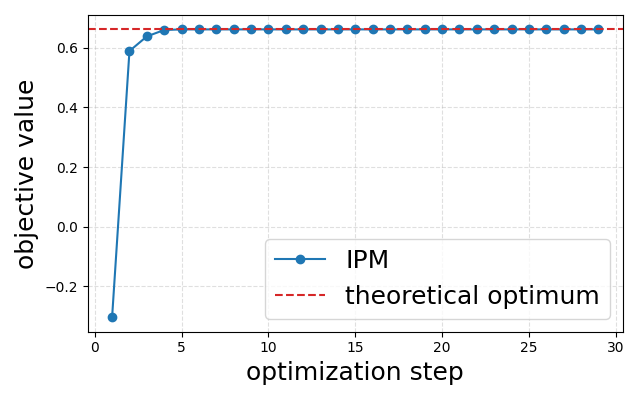
\includegraphics[width=\linewidth]{figs/obective_curve_p=0.5.png}
\subcaption{$p = 0.5$}
\end{subfigure}
\hfill
\begin{subfigure}[b]{.325\linewidth}
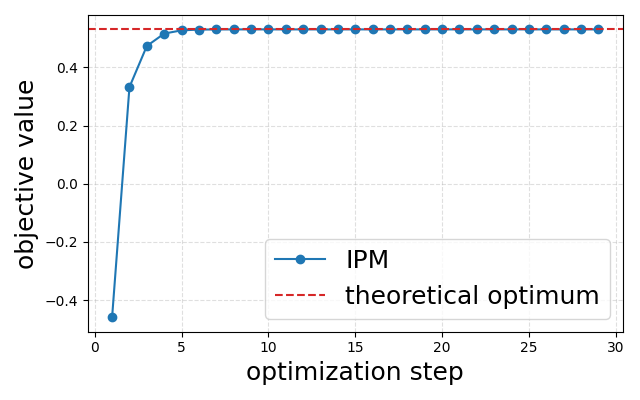
\includegraphics[width=\linewidth]{figs/obective_curve_p=0.75.png}
\subcaption{$p = 0.75$}
\end{subfigure}
\caption{Simulation of the two-token case for the log growth problem in Eq.~\eqref{eq:log-growth}. Three separate anchor distributions are used each with parameter $\delta = 0.01$. We solve the simplified maxmin problem using the CLARABEL interior point method solver which is run for $30$ steps. The theoretical optimum is computed as in Eq.~\eqref{eq:optimal-log-growth}.}
\label{fig:log-growth}
\end{figure*}


In this section, we verify our theoretical results with synthetic experiments on a family of simple target distributions.
Here, we consider the two-token case where $\lvert \cV\rvert = 2$ and for simplicity of notation, we let $\mathcal{V} = \{0,1\}$. Any anchor distribution we consider belongs to a one-parameter Bernoulli family $p_0 = \begin{bmatrix}
    p & 1-p
\end{bmatrix}$ for $p \in (0,1)$.
\paragraph{Log-growth optimality.}
We solve the optimization problem in Eq.~\eqref{eq:log-growth} numerically and compare the objective curve with the theoretical prediction.
With $n=2$, the problem can be simplified to the following maxmin problem:
$$\sup_e\sum_{v} p_0(v)\log e(v,v) + \frac{\delta}{2}\min\left\{\log \frac{e(0,1)}{e(1,1)}, \log \frac{e(1,0)}{e(0,0)}\right\}$$
subject to the constraint in Eq.~\eqref{eq:e-null} with $\cQ(p_0,\delta)$ replaced with the set of vertices $\cQ_{\text{ext}}(p_0,\delta) := \{p_0 \pm \frac{\delta}{2}(\mathbf{e}_0-\mathbf{e}_1)\}$. Using the CLARABEL interior point method solver \cite{Clarabel_2024}, we obtain the results in Fig. \ref{fig:log-growth}. We choose $\delta = 0.01$ and $p = 0.2,0.5,0.75$ corresponding to three separate anchor distributions $p_0$. For each $p_0$, we cold start the IPM solver and run it for $30$ steps with maximum allowed step size $0.99$. We observe that our numerical solution to Eq.~\eqref{eq:log-growth} converges to the proposed theoretical value in Eq.~\eqref{eq:optimal-log-growth}, hence verifying our theoretical results in the two-token case. 

\paragraph{Stopping time.}
In this setting, we simulate sequential testing with the optimal e-value $e^*$, as in Eq.~\eqref{eq:optimal-e}. Following Theorem \ref{thm:log-growth}, we let $\mathcal{A}^*$ be the adversary that chooses $q_t = q^*$ for all $t$ and $\cG^*$ be the generator that selects $w_t = w^*$ in response to $\mathcal{A}^*$ for all $t$. Under this setting, we simulate the stopping time over several $\alpha$ values to obtain the results in Fig. \ref{fig:stopping-time}. Here, we choose the parameters $\delta = 0.1$ and $p= 0.2,0.5,0.75$. For each anchor $p_0$, we compute the corresponding $q^*$, $w^*$, and $e^*$ using the closed-form equations in Theorem \ref{thm:log-growth}. We select $30$ values of $\alpha$ evenly log-spaced from $10^{-2}$ to $10^{-120}$. For each $\alpha$, we compute $10000$ stopping-times by generating sequences $(V^t,S^t)_{t \geq 1} \sim w^*$ and computing the resulting $\log e^*(V^t,S^t)$. We then average the stopping times to form an estimate of $\mathbb{E}_{\mu(\mathcal{A}^*,\cG^*)}[\tau_{\alpha}(e^*)]$. In Fig. \ref{fig:stopping-time}, we plot our estimates of $\mathbb{E}_{\mu(\mathcal{A}^*,\cG^*)[\tau_{\alpha}(e^*)]}/(\log(1/\alpha))$ which show that as $\alpha \downarrow 0$, the estimates converge to the theoretical rate of $1/J^*$, thereby validating the result in Theorem \ref{thm:stopping-time}.

\begin{figure*}[t]
\hfill
\begin{subfigure}[h]{.325\linewidth}
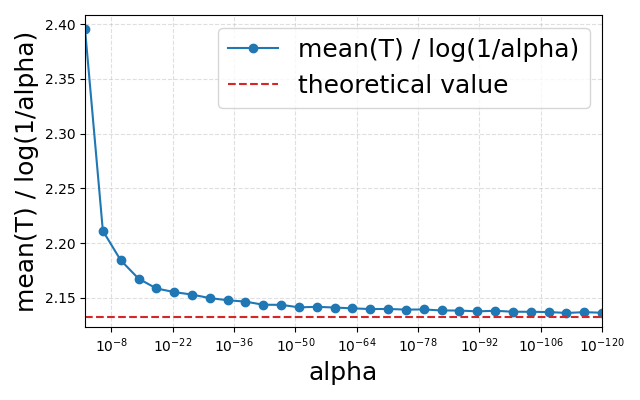
\includegraphics[width=\linewidth]{figs/stop_time_ratio_p=0.2.png}
\subcaption{$p = 0.2$}
\end{subfigure}
\hfill
\begin{subfigure}[h]{.325\linewidth}
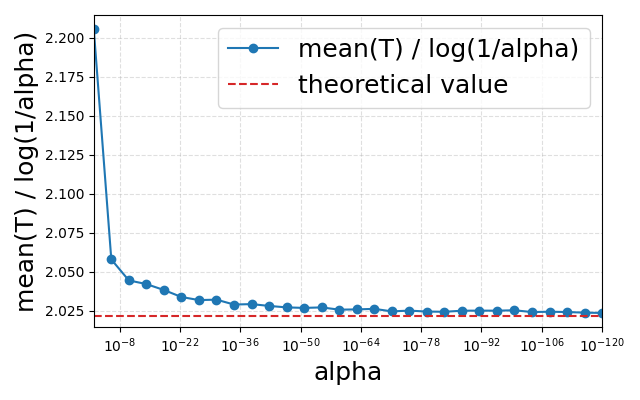
\includegraphics[width=\linewidth]{figs/stop_time_ratio_p=0.5.png}
\subcaption{$p = 0.5$}
\end{subfigure}
\hfill
\begin{subfigure}[h]{.325\linewidth}
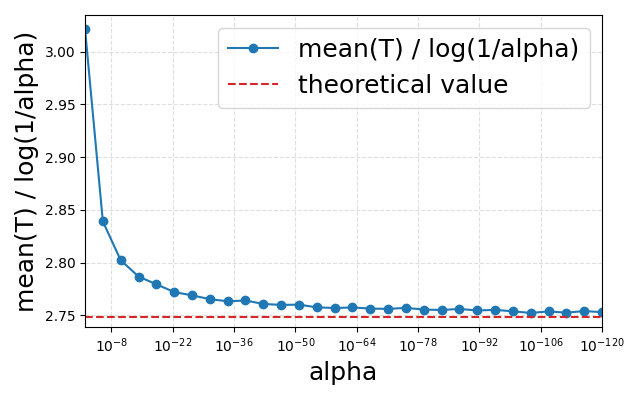
\includegraphics[width=\linewidth]{figs/stop_time_ratio_p=0.75.png}
\subcaption{$p = 0.75$}
\end{subfigure}
\caption{Simulation of the two-token case for the stopping time problem $\text{SC}(e^*)$. We simulate for three different anchor distributions $p_0 = \begin{bmatrix}
    p & 1-p
\end{bmatrix}$ with $\delta = 0.1$ and estimate average stopping times $\mathbb{E}[\tau_{\alpha}]$ for $\alpha$ values ranging from $10^{-2}$ to $10^{-120}$. Each $\mathbb{E}[\tau_{\alpha}]$ is estimated by simulating $10000$ stopping times $\tau_\alpha$. The plots above display graphs of $\frac{\mathbb{E}[\tau_\alpha]}{\log(1/\alpha)}$ with red dashed lines equal to $1/J^*$ where $J^*$ is as in Eq.~\eqref{eq:optimal-log-growth}. We observe that convergence to the theoretical optimum is obtained for sufficiently small $\alpha$.}
\label{fig:stopping-time}
\end{figure*}

\subsection{Experiments on real data}\label{sec:exp-real}

We evaluate the performance of our watermarking scheme in \Cref{thm:log-growth} by comparing it with several baselines on a real watermarking task.

\paragraph{Setup.}
We select Llama2-7B-chat~\citep{touvron2023llama} with temperature $0.7$ as target distribution (i.e., the model to be watermarked) and Phi-3-mini-128k-instruct~\citep{abdin2024phi3technicalreporthighly} as the anchor distribution. We evaluate our watermark using the \textsc{MarkMyWords} benchmark~\citep{piet2023mark}, which is an open-source benchmark designed to evaluate symmetric key watermarking schemes. 

\textsc{MarkMyWords} generates 300 outputs spanning three tasks---book summarization, creative writing, and news article generation---which mimic potential misuse scenarios. 
Then, watermarked outputs undergo a set of transformations mimicking realistic user perturbation or attacks: (1) character-level perturbations (contractions, expansions, misspellings and typos); (2) word-level perturbations (random removal, addition, and swap of words in each sentence, replacing words with synonyms); (3) text-level perturbations (paraphrasing, translating the output to another language and back).
Detection is run in a sequential test setting with early stopping. For baseline methods, we apply Bonferroni corrections to preserve \emph{anytime valid} Type-I error guarantees: let $p_k$ denote the p-value at time step $k \in \Z_+$, reject at the first time ${p_k} < \frac{\alpha}{k(k+1)}$.

\paragraph{Results.}

In this section, we present a comprehensive comparison of our method against these baselines in terms of quality and size. 
Quality measures the utility of the watermarked text. It is computed using Llama-3~\citep{dubey2024llama} with greedy decoding as a judge model, and ranges from zero to one.
{Size} represents the median number of tokens required to detect the watermark at a given p-value, computed over a range of perturbations listed above. All experiments enforce a Type-I error constraint of $\alpha = 0.02$. Lower values indicate higher efficiency.
We compare against five state-of-the-art watermarking schemes: 
``Distribution Shift''~\citep{kirchenbauer2023watermark}, 
``Exponential''~\citep{aaronson2022watermarking}, 
``Binary''~\citep{christ2023undetectable},
``Inverse Transform''~\citep{kuditipudi2023robust}, and ``SEAL''~\citep{huang2025watermarking}.

\begin{table}[h]
    \centering
    \begin{NiceTabular}{l|cc}
        \toprule
        {\bf Scheme
        } & {\bf Quality} ($\uparrow$) & {\bf Size} ($\downarrow$) \\
        \hline
        Exponential & 0.907	& $\infty$ \\
        Inverse Transform & 0.917 &	734.0 \\
        Binary & {\bf 0.919} &	$\infty$ \\
        Distribution Shift   & 0.912 &	145.0 \\
        SEAL   & 0.901 &	84.5 \\
        {\bf \Cref{thm:log-growth}} & {\bf 0.919} & {\bf 72.0} \\ 
        \bottomrule
    \end{NiceTabular}
    \vspace{.5em}
    \caption{{\fontfamily{ptm}\selectfont Comparison of our e-value-based watermarking scheme in \Cref{thm:log-growth} with baselines across quality and size. We report the median over different private keys and perturbation methods. The best result in each category is highlighted in bold. $\infty$ size suggests over half of the watermarked generations fail to be detected after perturbation. E-value-based watermarking demonstrates higher efficiency comparing with all baselines.}}
    \label{tab:comparison}
\end{table}

As shown in Table~\ref{tab:comparison}, our Anchored E-Watermarking framework significantly outperforms baseline methods in terms of detection efficiency while maintaining high generation quality. Specifically, our method improves over SEAL, confirming the superiority of the optimal e-value. Furthermore, we achieves nearly $2 \times$ speed improvement (from $145$ to $72.0$ tokens) compared to the best non-anchored baseline. Crucially, this efficiency gain does not come at the cost of text quality: the quality score of our method remains competitive with the baselines, demonstrating that E-value-based watermarking offers a superior trade-off between detectability and utility.
Due to space constraints, we defer additional experiment results to Appendix~\ref{sec:add_exp}.